\hypertarget{native_2lwip_2src_2apps_2snmp_2snmp__mib2__udp_8c}{}\section{/home/ayush/\+R\+I\+O\+T/tests/lwip/bin/pkg/native/lwip/src/apps/snmp/snmp\+\_\+mib2\+\_\+udp.c File Reference}
\label{native_2lwip_2src_2apps_2snmp_2snmp__mib2__udp_8c}\index{/home/ayush/\+R\+I\+O\+T/tests/lwip/bin/pkg/native/lwip/src/apps/snmp/snmp\+\_\+mib2\+\_\+udp.\+c@{/home/ayush/\+R\+I\+O\+T/tests/lwip/bin/pkg/native/lwip/src/apps/snmp/snmp\+\_\+mib2\+\_\+udp.\+c}}
{\ttfamily \#include \char`\"{}lwip/snmp.\+h\char`\"{}}\newline
{\ttfamily \#include \char`\"{}lwip/apps/snmp.\+h\char`\"{}}\newline
{\ttfamily \#include \char`\"{}lwip/apps/snmp\+\_\+core.\+h\char`\"{}}\newline
{\ttfamily \#include \char`\"{}lwip/apps/snmp\+\_\+mib2.\+h\char`\"{}}\newline
{\ttfamily \#include \char`\"{}lwip/apps/snmp\+\_\+table.\+h\char`\"{}}\newline
{\ttfamily \#include \char`\"{}lwip/apps/snmp\+\_\+scalar.\+h\char`\"{}}\newline
{\ttfamily \#include \char`\"{}lwip/udp.\+h\char`\"{}}\newline
{\ttfamily \#include \char`\"{}lwip/stats.\+h\char`\"{}}\newline
{\ttfamily \#include $<$string.\+h$>$}\newline
Include dependency graph for snmp\+\_\+mib2\+\_\+udp.\+c\+:
\nopagebreak
\begin{figure}[H]
\begin{center}
\leavevmode
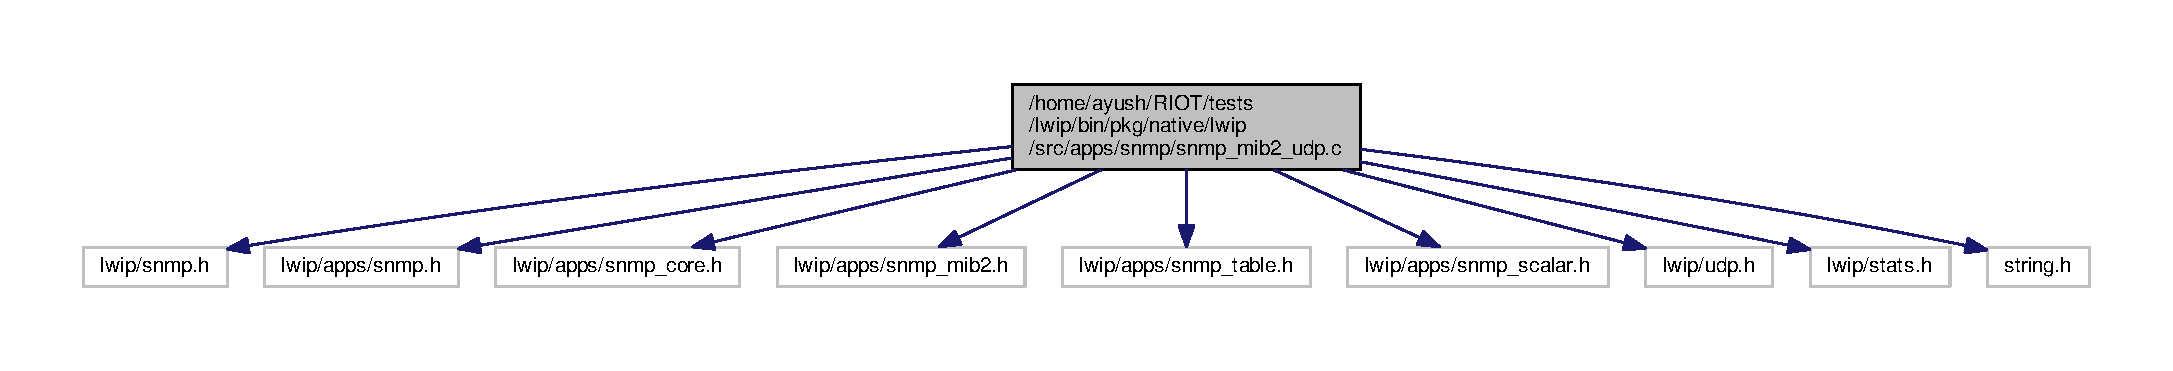
\includegraphics[width=350pt]{native_2lwip_2src_2apps_2snmp_2snmp__mib2__udp_8c__incl}
\end{center}
\end{figure}


\subsection{Detailed Description}
Management Information Base II (R\+F\+C1213) U\+DP objects and functions. 